\section{Commercial Systems}\label{sec:systems}
There are two main approaches of training CNNs for face recognition.

The first one is to train a multi-class classifier which can separate identities directly.
An example of such system is DeepFace~\ref{subsec:deepface}.

The second approach is to learn embedding using the triplet loss~\ref{sec:triplet-loss} function or similar.
FaceNet~\ref{subsec:facenet} is an example of a system being trained using the second approach.

\subsection{DeepFace}\label{subsec:deepface}
DeepFace~\cite{DeepFace} is a system developed by FaceBook Inc. in 2014.

The research is notable for its use of advanced alignment technique which consists of three steps:

\begin{enumerate}
    \item \textbf{2D Alignment}

    In this step the image is aligned in such a way that the fiducial points/landmarks are in a similar position
    to predetermined reference positions.
    To carry out this process it is first necessary to detect the 6 fiducial points/landmarks.
    These points and the reference positions are then used to find the parameters of an affine transformation.
    Applying the transformation to the original image gives us the desired result.
    \item \textbf{3D Alignment}

    In this step the image is warped onto a generic 3D shape model.
    This is achieved by localization of 67 fiducial points in the image and then fitting an affine
    camera\footnote{linear mathematical model to approximate the perspective projection followed by an ideal
    pinhole camera.} \textit{P} using the generalized least squares solution and the reference position $x_{3d}$ of
    points on the 3D shape model.

    \item \textbf{Frontalization}

    This is the final step and it consist of a computation and application of a piece-wise affine transformation T from
    $x_{2d}$ source to $\tilde{x_{3d}}$ target.
    The target $\tilde{x_{3d}}$ is a list of positions of reference fiducial points from the previous step enriched with
    residuals \textit{r}.
    These residuals were added to the reference positions $\tilde{x_{3d}}$ to account for non-rigid deformations which
    are not modeled by the affine camera \textit{P}.
    Without these residuals, all faces would be warped into the same shape losing important discriminative factors.
\end{enumerate}

\begin{figure}[H]
    \centering
    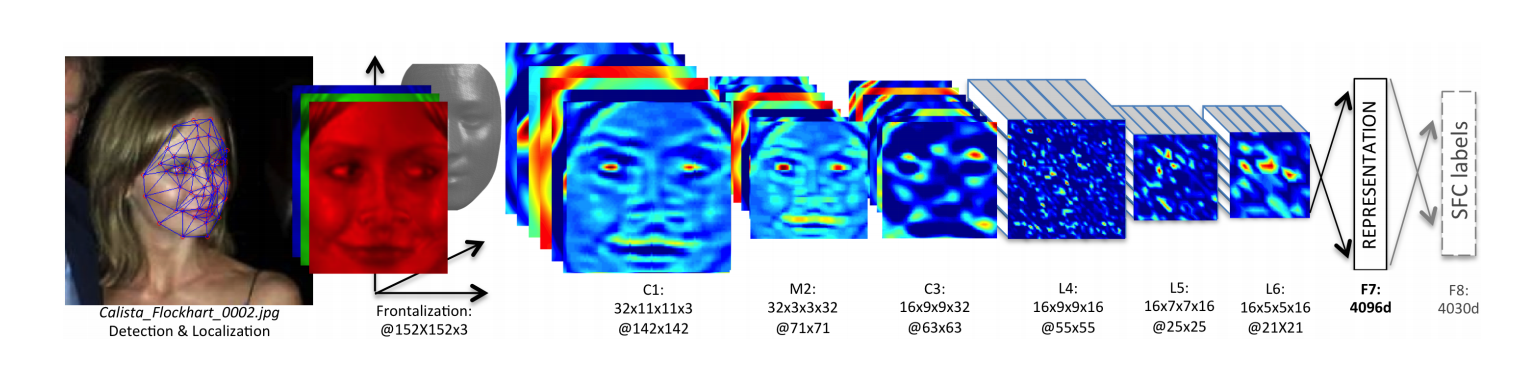
\includegraphics[width=\columnwidth]{images/face-recognition/deepface.png}
    \caption{Outline of DeepFace architecture~\cite{DeepFace}}
    \label{fig:deepface}
\end{figure}

There are 9 layers in the model with over 120 million parameters.
The process of classification is visualized in the picture~\ref{fig:deepface}.
The model was trained on more than 4 million images and as the name of the research paper~\cite{DeepFace} implies,
the results (\textbf{97.35\%} on LFW dataset~\ref{subsec:lfw}) almost matched the results of humans (\textbf{97.53\%}
on LFW dataset).


\subsection{FaceNet}\label{subsec:facenet}
FaceNet~\cite{FaceNet} is a system developed by researchers at Google Inc. in 2015.

An interesting innovation of FaceNet is the format of its output.
The output of the network is a vector representing a position in an euclidean space (so called embeddings) instead of a
number representing an identity.
This approach allows for straight-forward implementation of \textit{verification} and
\textit{identification}~\ref{ch:face-rec}.
Implementation of verification involves thresholding the distance between the reference and the newly obtained
embedding; and identification becomes k-NN classification problem.

\begin{figure}[H]
    \centering
    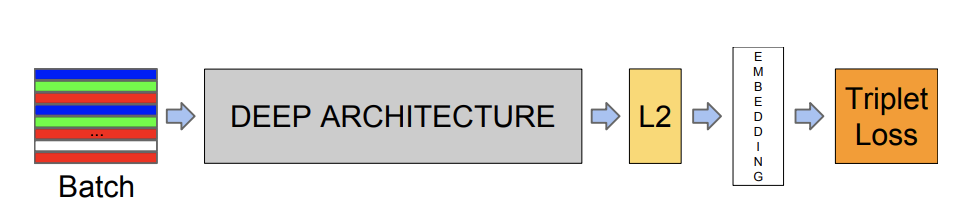
\includegraphics[width=\columnwidth]{images/face-recognition/facenet.png}
    \caption{Outline of FaceNet architecture~\cite{FaceNet}}
    \label{fig:facenet}
\end{figure}

The loss function used to train the model is called \textit{triplet loss}~\ref{sec:triplet-loss}.
Researches at Google came up with a new online method\footnote{Training samples are selected during training.} which
ensures that the difficulty of triplets is rising as the network trains.

The advantages of the model are its accuracy and the compactness of the face representation.
The accuracy exceeded that of human with \textbf{99.63\%} on LFW dataset~\ref{subsec:lfw} and the euclidean space has
only 128 dimensions.

Another advantage is how well the model handles faces which are not in ideal position.
This removed the need for complex preprocessing and face frontalization.
To use proper terms the system is \textit{pose invariant}.